% compilation using latex (i.e. via a ps file)
% \documentclass[a4paper,11pt,twoside,openright,dvips]{book}

% compilation using PDFLATEX - Note that pdflatex is known to have issues with
% some of the pstricks-packages
\documentclass[a4paper,11pt,pdftex,oneside]{book}

%%%%%%%%%%%%%%%%%%%%%%%%%%%%%%%%%%%%%%%%%%%%%%%%%%%%%%%%%
% Input info. for cover, titlepages, pdf properties, version etc.
%%%%%%%%%%%%%%%%%%%%%%%%%%%%%%%%%%%%%%%%%%%%%%%%%%%%%%%%%

\def\ThesisAuthor{Anders Bahnsen\\Aleksander Gosk\\Kim Rostgaard Christensen}
                         %multiple authors separated by "\\"
                         %If there are multiple authors adjust the \vspace 
                         %in thesislayout.sty as necessary 

\def\ThesisAuthorForHyperref{Anders Bahnsen,Aleksander Gosk,Kim Rostgaard Christensen}
                                %list of authors for pdf
                                %properties. Multiple authors separated by ","

\def\ThesisTitle{31070} %project title
\def\Subtitle{Hands-on mikrocontroller programmering} %subtitle - if any

\def\thesiskeywords{latex template, other keywords} %keywords for the pdf file

\def\thesissubject{} %only for pdf properties - doesn't appear on printed
                     %versions

\def\Supervisor{Preben Nyeng} %list of supervisors. multiple
                                %supervisors are separated by "\\"
\def\projecttype{3 week project report, January 2010} %type of project (see README file
                                %for explanation)
\def\ISBNNUMBER{} %type \ISBNNUMBER{ISBN: xxx} if your project has one
\def\DatePublished{22. January 2010} %date of publication
\def\Klasse{1 (public)} %project class (see README file for explanation)
\def\Degree{} %obtained degree (see
                                %README file for explanation)
\def\ECTSpoints{5} %# of ECTS points 
\def\Udgave{First} %edition
\def\Owner{Group 6, 2010} %name of copyright and year

\def\thesisversion{final} %OBSOBS choose this for final version (official set of
                          %title pages) 
%\def\thesisversion{draft} %OBSOBS choose this for draft version (simple title
                           %page and no info page

\def\thesislinks{no}%OBSOBS choose this for paper version 
%\def\thesislinks{yes}%OBSOBS choose this for online version 

\def\thesislanguage{en}%OBSOBS compile document for English 
%\def\thesislanguage{da}%OBSOBS compile document for Danish

%do NOT modify
\def\danishlang{da}
\def\printversion{final}

%%%%%%%%%%%%%%%%%%%%%%%%%%%%%%%%%%%%%%%%%%%%%%%%%%%%%%%%%
% Load style definitions, packages, etc. 
%%%%%%%%%%%%%%%%%%%%%%%%%%%%%%%%%%%%%%%%%%%%%%%%%%%%%%%%%

%load thesisdef and styles
\usepackage{thesisdef}
\usepackage{graphics}

\begin{document}

%%%%%%%%%%%%%%%%%%%%%%%%%%%%%%%%%%%%%%%%%%%%%%%%%%%%%%%%%
% FRONT MATTER
%%%%%%%%%%%%%%%%%%%%%%%%%%%%%%%%%%%%%%%%%%%%%%%%%%%%%%%%%

\frontmatter

\ifx\thesisversion\printversion
% for final version include standard dtu cover pages
%\pagenumbering{alph}%dummy numbering for pdf-file (numbering set as a
                    %pdf-property and is NOT visible on the document). The
                    %hyperref package complains if duplicate numbering exists

\coverpages         %generate the first four pages
\else
  %for draft version use simple title page
\title{\ThesisTitle{} - \Subtitle{}}
\author{\ThesisAuthor}
%\thispagestyle{empty}
\maketitle
%\newpage
%\thispagestyle{empty}
\fi



%%%%%%%%%%%%%%%%%%%%%%%%%%%%%%%%%%%%%%%%%%%%%%%%%%%%%%%%%
% TOC,LOF,LOT and SETUP HEADER
%%%%%%%%%%%%%%%%%%%%%%%%%%%%%%%%%%%%%%%%%%%%%%%%%%%%%%%%%

%\newpage
\tableofcontents 
\pagestyle{fancyplain}%enable headers in the main document
%\chaptermark{Contents}
%\renewcommand{\sectionmark}[1]{\markright{#1}}
%\sectionmark{Contents}
%\newpage

%%%%%%%%%%%%%%%%%%%%%%%%%%%%%%%%%%%%%%%%%%%%%%%%%%%%%%%%%
% MAIN CHAPTERS INCLUDE
%%%%%%%%%%%%%%%%%%%%%%%%%%%%%%%%%%%%%%%%%%%%%%%%%%%%%%%%%

\mainmatter

\setcounter{page}{1}\pagenumbering{arabic} %\pagestyle{fancyplain}

\chapter{Introduction}
This report documents the design and implementation of a travel agency service The travel agency acts as a coordinator by composing and synchronizing bookings and accounts from third party actors.

\section{Introduction to Web Services}
The current trend within distributed systems is using the world wide web and it's technologies as a transportation and encapsulation layer. As these technologies are standardized, interoperability becomes less of a hassle than if every protocol should be implemented from scratch.\\\\
From the times where first static web pages emerged in the new World Wide Web, upto now, a big evolution process has taken place. This process may be described best as; chaotic. Everyone that has done web programming within the last 10 years will flee in terror by pronouncing to them the letters IE.\\
But, that aside, from this evolution it became clear that standards should drive the web forward - as they had from the days of HTTP 0.9. And as web applications grew larger and became increasingly dynamic and intercoupled, it also became clear that interfacing was a lot more problematic than what could be handled \emph{ad-hoc}.\\\\
The following section is a description of some of the key technologies we will use in this report, along with a brief discussion on some of the objective strengths and weaknesses.

\begin{description}
\item[HTTP] The \textbf{H}yper\textbf{T}ext \textbf{T}ransfer \textbf{P}rotocol is a plaintext stateless request-response protocol with standardized methods and response codes. It is deployed everywhere, from coffee machines to mainframes and thus a robust technology to base a web application on. Most programming languages have auxiliary libraries that provide both HTTP client and server components for re-use.

\item[XML] The e\textbf{X}tensible \textbf{M}arkup \textbf{L}anguage is a subset of the Standard Generalized Markup Language (SGML) and has a very famous cousin named Hypertext Markup Language - or HTML. XML is, basically, a general purpose markup language for adding semantics to documents. This semantic is further formalized by either linking a Document Type Definition (DTD), or an XML Schema (XSL) to the document. A large advantage of XML is that it, like HTTP, is a widely used standard, and most programming languages have libraries for using XML without having to parse everything. XML - being a generalized language - has the further advantage that you can build new standards as XML applications and inherit the well-formedness\footnote{Grammatically and semantically correct.} property of of XML itself, and the general XML parser can used.

\item[WSDL] \textbf{T}he \textbf{W}eb \textbf{S}ervice \textbf{D}efinition Language is an XML application introducing formalism to web application in an attempt to unify the diverging methods for collaborating via web.

\item[SOAP] \textbf{S}hoddy \textbf{O}verbloated \textbf{A}ccess \textbf{P}rotocol is another XML application % Simple Object Access Protocol
SOAP is independent of HTTP, and can therefore not inherit any information deriving from HTTP headers - even if used over HTTP.

\item[BEPL] \textbf{B}ullshit \textbf{P}olluted \textbf{E}xecution \textbf{L}anguage %Business Process Execution Language is also an XML application
%TODO Should we discuss this one, or just mention it in the bank interface section? \item[UDDI/service discovery]

\item[REST] The concept \textbf{RE}presentational \textbf{S}tate \textbf{T}ransfer covers the architecture defined by Roy Fielding and is specific application to HTTP (1.1) and centralized around the concept of resources and representations\footnote{Typically states of resources}. Resources are accessed and changed by ordinary HTTP methods: GET, PUT, POST, DELETE and standard HTTP 1.1 response codes are used to explain to the caller how the request went. For instance, a DELETE operation on a non-existing ID could return a 404 - Not Found, while it would return 200 - OK if all went well. There exists no (standardized) formalization language to describe RESTful web services, like there does with WSDL.

\item[JSON] \textbf{J}ava\textbf{S}cript \textbf{O}bject \textbf{N}otation is an object serialization language that is human-readable -- much like XML. One of the big advantages of JSON over XML is, however, that grammer, and thus effectively, the parser is very simple. It is also less verbose than XML and therefore has less overhead. It has draft support for schemas, and has currently no general way of validating data, or enforcing constraints. Due to its simple nature, it doesn't support any other types than the ones that are built-in. JSON is typically used in web applications, and in strong collaboration with the REST paradigm.

%TODO Find reference to XML book and course book.
\end{description}
\chapter[Requirements]{Requirements analysis and specification}
\label{chap:requirements}
%ELSAM states that we should be sensitive to changes in the powergrid frequency, and be able to communicate using a network.
The ELSAM agreement states that the grid frequency at all times must be 50Hz. If the values goes lower, our device should turn off unneeded devices. ELSAM defines two types of loads; Normal operation reserve and Disturbance reserve.\\
The Normal operation reserve should off-load when the frequency drops 49.9Hz, and shut off equipment able to do so in 2-3 minutes or less, not crucial to production (e.g. heater or lighting).\\ 
Disturbance reserve mode is used when the grid frequency does not return to normal state. In our case we turn off a battery powered device (a laptop) and try to make sure we dont empty their batteries completely before getting the power back.

\begin{figure}[!h]
  \centering
  \label{fig:reserver_demands}
  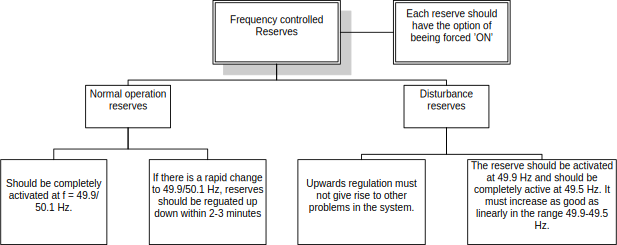
\includegraphics[width=0.9\textwidth]{figs/Demands_for_automatic_active_reserves.pdf}
  \caption{Hierarchy of the frequency controlled reserves in this report}
\end{figure}
To be able to do more ``intelligent'' grid-off loading, we must be able to communicate with the outside world. As there is no protocol specified, the logical choice would be tcp/ip for transport, as there is is already a well-established global infrastructure using this. The data should be transferred in an easy parsable format, such as XML.\\\\
Users of the device should also be able to view the status, current configuration and make changes to the configuration as well. The status and configuration should be available both from a physical interface and via a remote interface. As out device has a touchscreen it will serve the purpose as a physical interface, and the remote interface should be done in html.\\\\
This leaves us with the following requirements:
\begin{itemize}
\item Detect grid frequency, and respond to changes
\item Toggle relays based on frequency algorithm
\item Implement a TCP/IP stack
\item Implement a HTTP server
\item Design human interfaces for local access
\item Design human interfaces for remote access
\item Design machine interfaces for remote access
\end{itemize}

\section{Tools used}
An application development process' success or failure can depend largely on the tools used in the process. Good tools for documenting, debugging and versioning should be considered bare minimums.
\subsection{Debugging tools and methods}
When developing the communications interface we use the program ``wireshark'' \footnote{www.wireshark.org} to verify http requests and responses.\\
The board we will be using contains a JTAG port, for interactive debugging. This means we are able to stop the processor, read and modify registers or memory. This feature is extemly useful when debugging an application.

\subsection{Information scraping}
For doing quick notes on random information concerning code, documentation, requirements or specifications. We will be using a wiki for this purpose

\subsection{Versioning}
When developing an application, a versioning system is very useful both for experimenting with new features, because you have the ability to quickly roll-back to a working version. It is also a great way to do backup on your project.

%\section{Chapter Summary}  %% Should this be here ?
%\label{sec:SummaryChap2}




\documentclass[10pt,a4paper]{article}
\usepackage[utf8]{inputenc}
\usepackage{url}
\usepackage{amsmath}
\usepackage{amsfonts}
\usepackage{amssymb}
\usepackage{listings}
\usepackage{graphicx}

\usepackage{color}

\def\File#1{\textsf{#1}}
\def\Code#1{\texttt{#1}}
\def\Key#1{\textsf{#1}}

\definecolor{mygreen}{rgb}{0,0.6,0}
\definecolor{mygray}{rgb}{0.5,0.5,0.5}
\definecolor{mymauve}{rgb}{0.58,0,0.82}

\lstset{ %
  backgroundcolor=\color{white},   % choose the background color; you must add \usepackage{color} or \usepackage{xcolor}
  basicstyle=\footnotesize,        % the size of the fonts that are used for the code
  breakatwhitespace=false,         % sets if automatic breaks should only happen at whitespace
  breaklines=true,                 % sets automatic line breaking
  captionpos=b,                    % sets the caption-position to bottom
  commentstyle=\color{mygreen},    % comment style
  deletekeywords={...},            % if you want to delete keywords from the given language
  escapeinside={\%*}{*)},          % if you want to add LaTeX within your code
  extendedchars=true,              % lets you use non-ASCII characters; for 8-bits encodings only, does not work with UTF-8
  frame=single,                    % adds a frame around the code
  keywordstyle=\color{blue},       % keyword style
  language=Octave,                 % the language of the code
  morekeywords={*,...},            % if you want to add more keywords to the set
  numbers=left,                    % where to put the line-numbers; possible values are (none, left, right)
  numbersep=5pt,                   % how far the line-numbers are from the code
  numberstyle=\tiny\color{mygray}, % the style that is used for the line-numbers
  rulecolor=\color{mygray},         % if not set, the frame-color may be changed on line-breaks within not-black text (e.g. comments (green here))
  showspaces=false,                % show spaces everywhere adding particular underscores; it overrides 'showstringspaces'
  showstringspaces=false,          % underline spaces within strings only
  showtabs=false,                  % show tabs within strings adding particular underscores
  stepnumber=2,                    % the step between two line-numbers. If it's 1, each line will be numbered
  stringstyle=\color{mymauve},     % string literal style
  tabsize=2                       % sets default tabsize to 2 spaces
%  title=\lstname                   % show the filename of files included with \lstinputlisting; also try caption instead of title
}

\title{01435 Practical Cryptanalysis\\Project 3}
\author{Kim Rostgaard Christensen - s084283}
\begin{document}
\maketitle
\begin{abstract}
The purpose of this report is to document the tool developed for decrypting cipher-text and recovering keys generated with the Linear Congruence Generator from GCC (old glibc).\\
Full sources can be found at:\\
 \url{https://github.com/rostgaard/practical_cryptoanalysis/}
\end{abstract}

\section*{Project description}
A file with ciphertext, a description of the key generation, and an approximate date of key generation, which is used as seed, is given.\\
The purpose is then to implement a tool that decrypts ciphertext.

\section*{Design and implementation}
The first step of the tool will be to generate the keys needed for decrypting. Validation can be done by detecting non-printable characters. For speed purposes, only the first 16 bytes will be decrypted in the evaluation step.\\
For the implementation the package \Code{Ada.Streams.Stream\_IO} was used to read in files. This enables us to treat a file as a stream - enabling us to read raw bytes without being affected by control signals. In this tool, the entire buffer is read to memory - but could just as easily be streamed in chunks.\\
Every key is generated in a hashed map, so we can ensure uniqueness of the keys. At the end  of key generation, every key is checked using the non-printable-characters-check.
\section*{Usage}
The tool is command-line only, and take at least one parameter; the path to the ciphertext tile.\\
You can also give the tool an additional argument which is the maximum keys it should try to find. For this case, 256 is enough, and we can quit early. Giving no arguments will result in a ``usage'' description printed to the command line.

\section*{Observations}
During development, one thing became apparent: There were only 256 distinct keys.\\
Investigating further, we found that every byte value occurred exactly 16 times, and once in every index. Diving the keys into two halves and plotting them, gives the pattern shown in figure \ref{fig:scatter_plot}.
\begin{figure}[h]
\includegraphics[scale=0.45]{../output/scatter.pdf}
\caption{MSB/LSB plot}
\label{fig:scatter_plot}
\end{figure}


\section*{Further work}
If the keyspace is large, it may be infeasible to save all unique keys prior to trying them. Instead of trying all keys, a large LRU\footnote{Least Recently Used} buffer could hold the latest tried ones.
\end{document}
\chapter{Conclusion}
\label{chap:conclusion}
In the beginning of the project we spent a great deal of time cleaning and refactoring code, making it more modulary and easy to navigate. But as the application evolved and grew in size and complexity, it became increasingly difficult to maintain a consistency in the code. Espeacially when thing were not doing as planned. New code arose in places where it did not belong.\\
From this we have learned about the importance of defining a clear program structure and functionality from the start of the project, and enforcing it thoughout the development process.\\\\
The webserver is responding slowly, but is very functional. The xsl transformations works like a charm in modern browsers and should definitly be considered in the case of an official http+xml implementation.\\\\
The LCD screen, acting as both in- an output, gives a quick way of getting an overview of the current status of the system. As well as modifying the system paramters realtime.\\ The values displayed are a bit off, due to programming errors. But it gives you an idea on how a finished system should look and behave.


%\input{appendix.tex} 



\end{document}
